\begin{enumerate}[label=\thesection.\arabic*.,ref=\thesection.\theenumi]
\numberwithin{equation}{enumi}

\item For an LTI system, the Bode plot for its gain defined as
\begin{align}
	G(s) = 20\log\abs{H(s)}
	\label{eq:ee18btech11001_gain}
\end{align}
is as illustrated in the Fig. \ref{fig:ee18btech11001_bode}. Express $G(f)$ in terms of $f$.\\
\begin{figure}[ht!]
    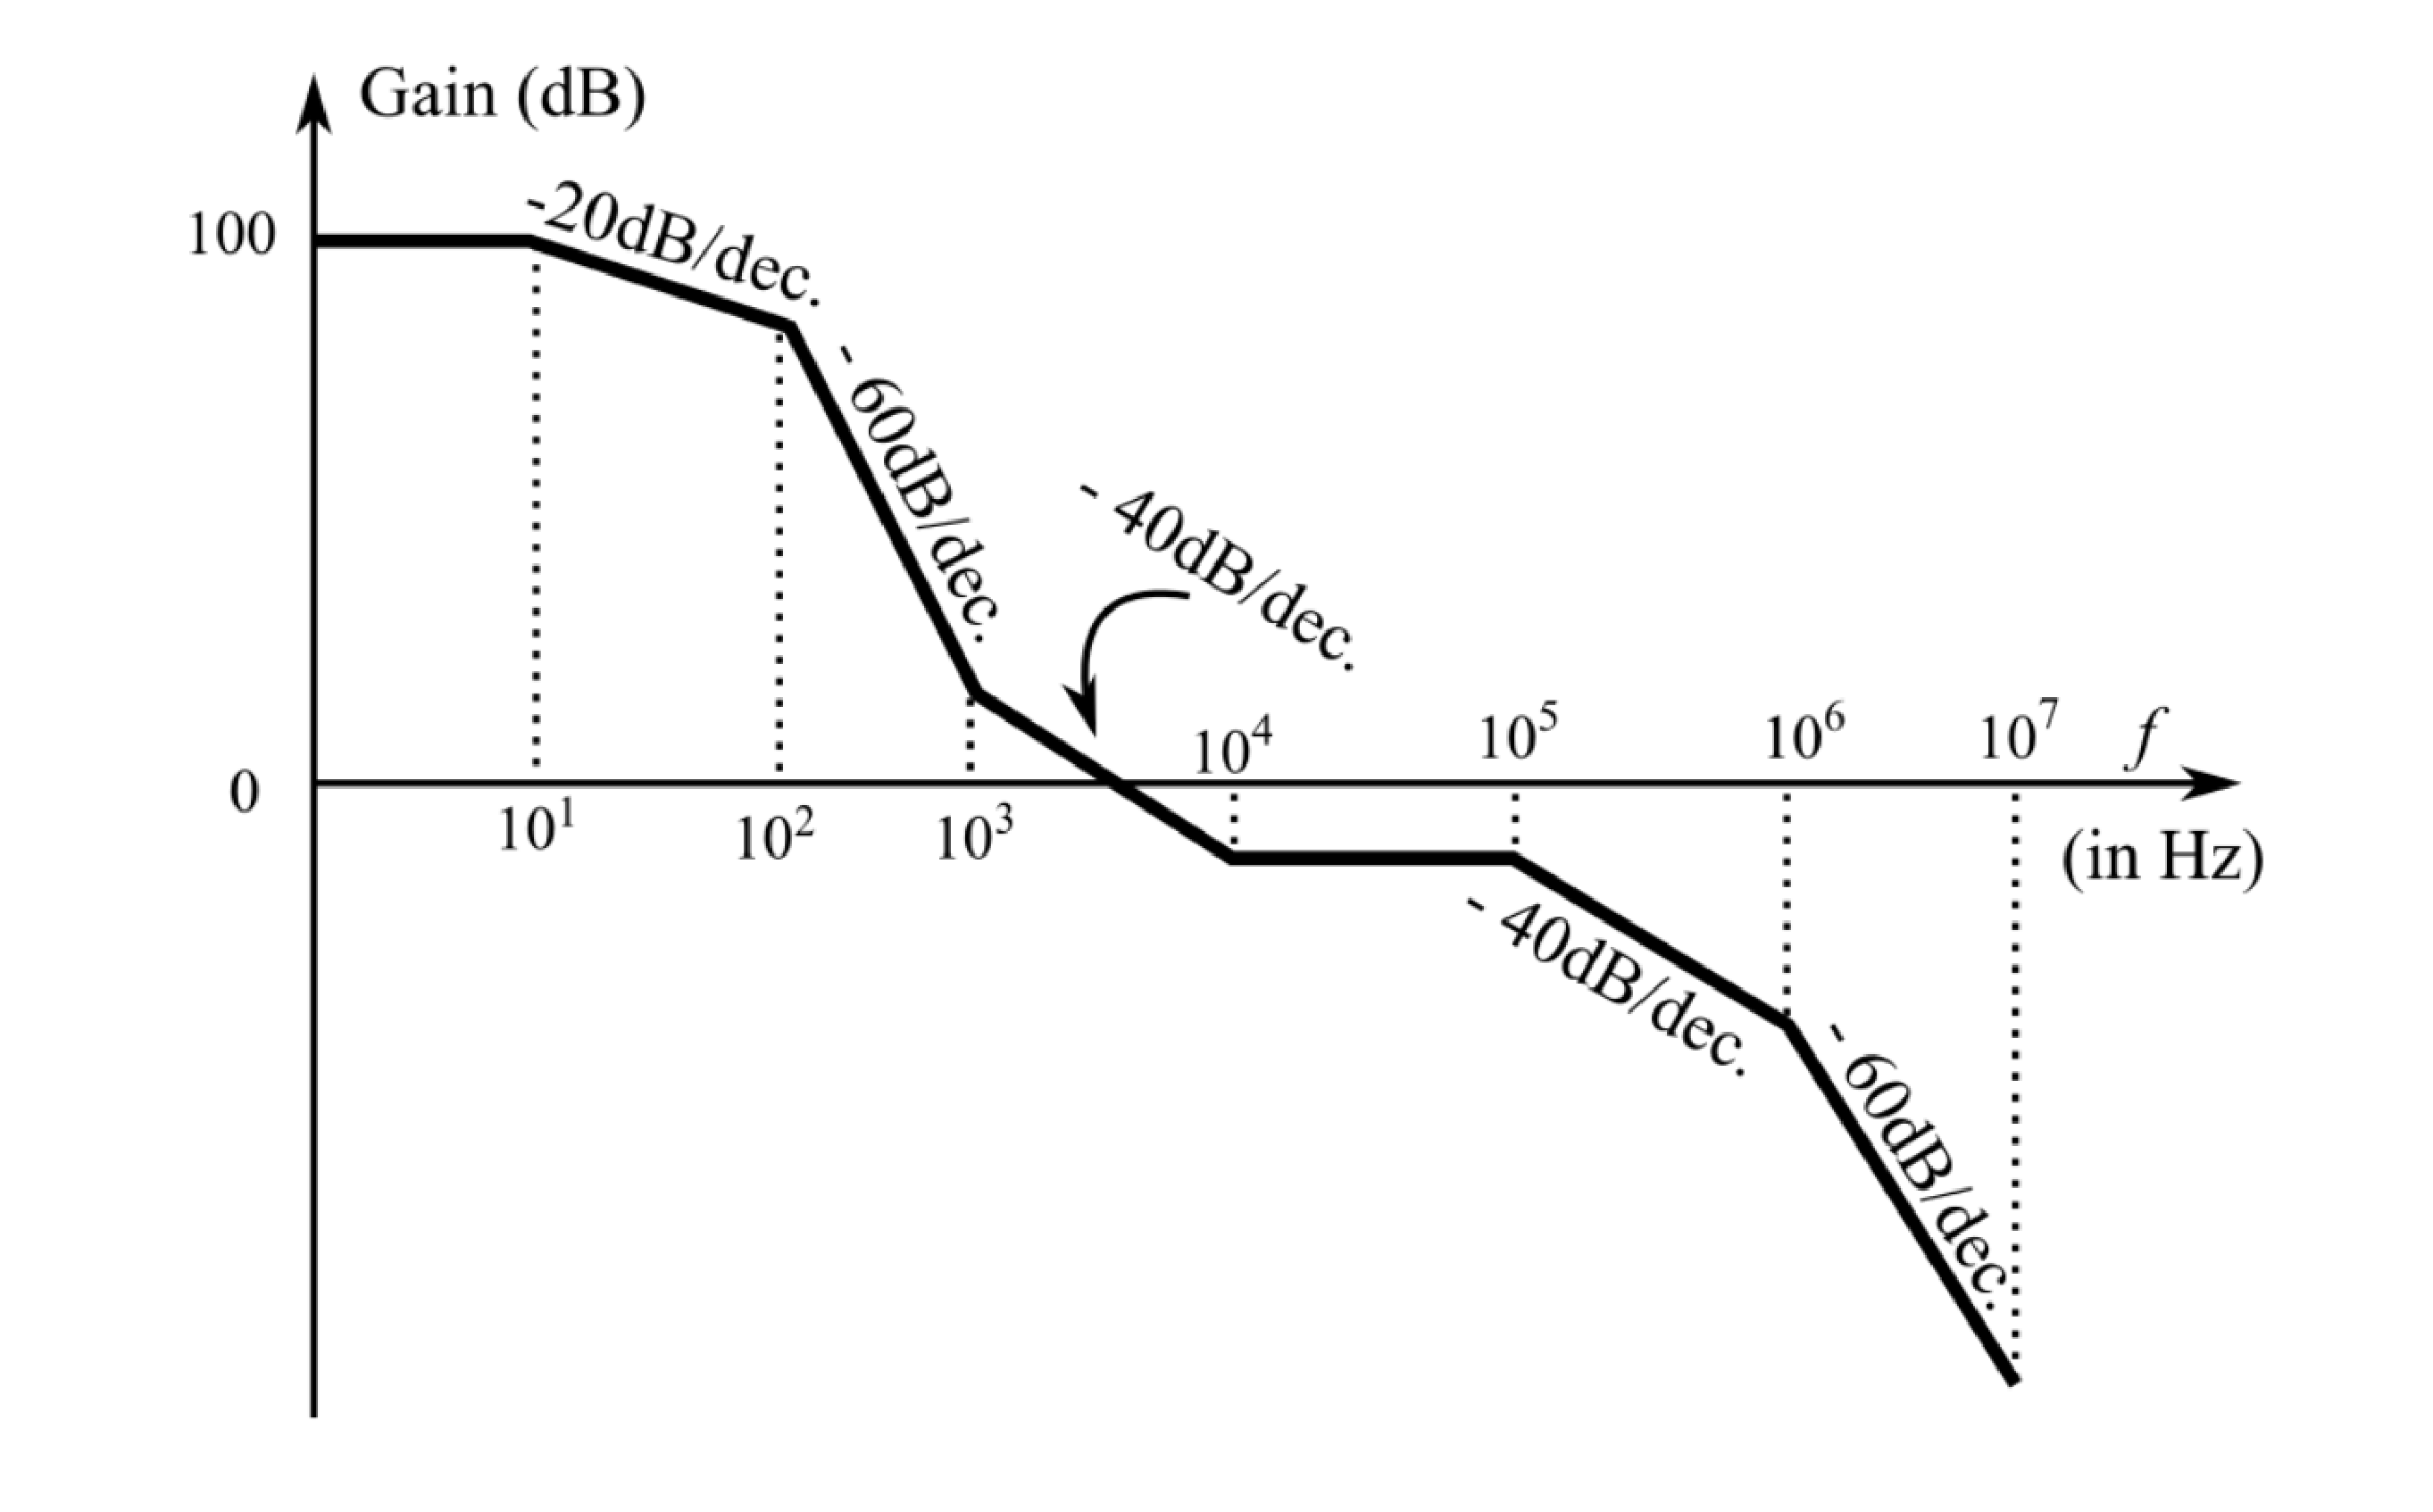
\includegraphics[width=\columnwidth]{./figs/ee18btech11001.eps}
    \caption{}
    \label{fig:ee18btech11001_bode}
\end{figure}\\

\solution
\begin{align}
 G(f) = 
 \begin{cases} 
        100 & 0 < f < 10^{1} \\
      120-20log(f) & 10 < f < 10^{2} \\
      200-60log(f) & 10^2 < f < 10^{3} \\
      140-40log(f) & 10^{3} < f < 10^{4} \\
       -20 & 10^{4} < f < 10^{5} \\
      180-40log(f) & 10^{5} < f < 10^{6} \\
      300-60log(f) & 10^{6} < f < 10^{7}   
 \end{cases}
\end{align}

%-----------------------------------------------------------------------%

\item Express the slope of $G(f)$ in terms of $f$.
\\
\solution\\
\begin{align}
Slope = \nabla G(f) &= \dfrac{d(G(f))}{d(log(f))}
\end{align}

\begin{align}
 \nabla G(f) = 
 \begin{cases} 
        0 & 0 < f < 10^{1} \\
      -20 & 10 < f < 10^{2} \\
      -60 & 10^{2} < f < 10^{3} \\
      -40 & 10^{3} < f < 10^{4} \\
       0 & 10^{4} < f < 10^{5} \\
      -40 & 10^{5} < f < 10^{6} \\
      -60 & 10^{6} < f < 10^{7}   
 \end{cases}
\end{align}

%-----------------------------------------------------------------------%

\item Express the change of slope of $G(f)$ in terms of $f$.
\\
\solution\\
$\Delta(\nabla G(f))$  = Change of slope G(f) at f

\begin{align}
 \Delta(\nabla G(f)) = 
 \begin{cases} 
      -20 &  f = 10^{1} \\
      -40 &  f = 10^{2} \\
      +20 &  f = 10^{3} \\
      +40 &  f = 10^{4} \\
      -40 &  f = 10^{5} \\
      -20 &  f = 10^{6} 
 \end{cases}
\end{align}

%-----------------------------------------------------------------------%

\item Find the number of poles and zeros of $H(s)$.
\\
\solution \\
\textbf{When a zero is encountered the slope always increases by 20 dB/decade}\\
\textbf{When a pole is encountered the slope always decreases by 20 dB/decade}
\begin{align}
	N_{p} = 6  
\end{align}
\begin{align}
	N_{z} = 3
\end{align}

%-----------------------------------------------------------------------%

\item Find the location of the poles and zeros of $H(s).$The number of system poles $N_{p}$ and number of system zeros $N_{z}$ in the frequency range 1 Hz $\leq$ f $\leq$ $10^{7}$ Hz is.
\\
\solution\\
\textbf{When a zero is encountered the slope always increases by 20 dB/decade}\\
\textbf{When a pole is encountered the slope always decreases by 20 dB/decade}

So, Poles are encountered at\\ $f = 10,10^2,10^5,10^6$\\
Similarly Zeros are encountered at\\ $f = 0,10^3,10^4$

%-----------------------------------------------------------------------%

\item Obtain the transfer function of $H(s)$.
\\
\solution\
Let us consider a generalized transfer gain\\
\begin{align}
	H(s) = k \dfrac{(s-z_{1})(s-z_{2})...(s-z_{m-1})(s-z_{m})}{(s-p_{1})(s-p_{2})....(s-p_{n-1})(s-p_{n})}
\end{align}\\
\begin{multline}
	Gain = 20\log\abs{H(s)} = 20\log \abs{k} + 20\log \abs{s-z_{1}} 
	    \\
	    + 20\log \abs{s-z_{2}} + \dots + 20\log \abs{s-z_{m}} - 20\log \abs{s-p_{1}} 
	    \\
	    - 20\log \abs{s-p_{2}} - \dots - 20\log \abs{s-z_{n}} 
\end{multline}\\

Let us consider the term $ 20\log \abs{s-z_{1}} $ and let $s = j\omega$\\
\begin{align}
	20\log \abs{s-z_{1}} = 20\log \abs{\sqrt{\omega^{2} + z_{1}^{2}}}
\end{align}\\

Based on log scale plot approximations,to the left of $z_{1} \hspace{5pt} \omega << z_{1}$ and towards right  $\omega >> z_{1}$\\
For $\omega < z_{1}$\\
\begin{align}
	20\log \abs{s-z_{1}} = 20\log \abs{\sqrt{\omega^{2} + z_{1}^{2}}}
	&= 20 \log \abs{z_{1}}\\
	&= constant
\end{align}  
i.e. Slope = 0\\

For $\omega > z_{1}$

\begin{align}
	20\log \abs{s-z_{1}} = 20\log \abs{\sqrt{\omega^{2} + z_{1}^{2}}} = 20 \log \abs{\omega} 
\end{align}

i.e Slope = 20\\

\textbf{When a zero is encountered the slope always increases by 20 dB/decade}\\
By performing similar analysis for $-20\log \abs{s-p_{1}}$, we conclude that\\
\textbf{When a pole is encountered the slope always decreases by 20 dB/decade}
\\
So, Poles are encountered at $f = 10,10^2,10^5,10^6$\\
Similarly Zeros are encountered at $f = 0,10^3,10^4$

Final Transfer function is\\
\begin{align}
	H(f) = \dfrac{K(f+10^{3})(f+10^{4})^{2}}{(f+10^{1})(f+10^{2})^{2}(f+10^{5})^{2}(f+10^{6})}
\end{align}\\
\begin{align}
\begin{small}
	G(f) = 20\log\dfrac{K(f+10^{3})(f+10^{4})^{2}}{(f+10^{1})(f+10^{2})^{2}(f+10^{5})^{2}(f+10^{6})}
\end{small}
\end{align}

$ s = j\omega = j2\pi f$
\begin{align}
\begin{small}
	H(s) = \dfrac{K(s+j2\pi 10^{3})(s+j2\pi 10^{4})^{2}}{(s+j2\pi 10^{1})(s+j2\pi 10^{2})^{2}(s+j2\pi 10^{5})^{2}(s+j2\pi 10^{6})}
\end{small}
\end{align}\\

%-----------------------------------------------------------------------%

\item Obtain the Bode plot and the slope plot for $H(s)$ and verify with  Fig. \ref{fig:ee18btech11001_bode}
\\
\solution
Bode Plot of obtained Transfer Function is 
\begin{figure}[htp]
    \centering
    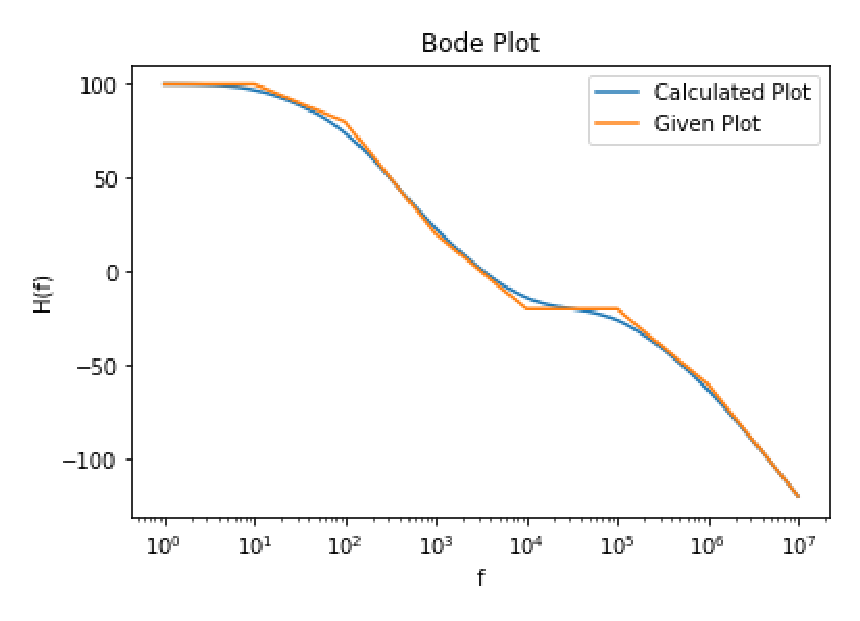
\includegraphics[width=\columnwidth]{./figs/ee18btech11001_2.eps}
    \caption{}
    \label{fig:bode}
\end{figure}

\end{enumerate}
